In the previous section, time was supposed to be continuous. In this new chapter however, we will regard time as a discrete variable meaning that we consider fixed size time intervals for our inventory management study. To each of these periods corresponds a certain demand, denoted $d_i$ for period $i$, and a decision (called "action") that we take in order to satisfy the demand, denoted $a_i$. We represent this situation with plots similar to figure (\ref{periodic:plot}) where each box stands for a period of time. The question we have to answer in this chapter is : "What actions do I have to take in order to fulfill the demand minimizing the total cost ?", or similarly : "How many items $a_i$ should I buy in period $i$ to minimize the cost ?"

\begin{figure}[h!]
    \centering
    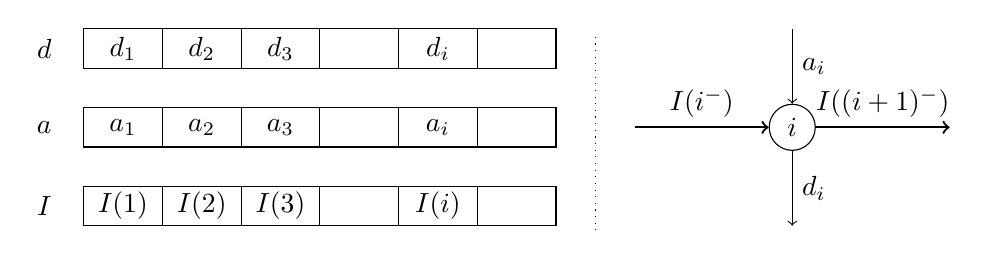
\begin{tikzpicture}
        \draw (.5, .25) node {$d$};
        \foreach \x/\t in {1/$d_1$, 2/$d_2$, 3/$d_3$, 4/$\hdots$, 5/$d_i$, 6/$\hdots$} {
            \draw (\x, 0) rectangle (\x+1, .5);
            \draw (\x+.5, .25) node {\t};
        }

        \draw (.5, -.75) node {$a$};
        \foreach \x/\t in {1/$a_1$, 2/$a_2$, 3/$a_3$, 4/$\hdots$, 5/$a_i$, 6/$\hdots$} {
            \draw (\x, -1) rectangle (\x+1, -.5);
            \draw (\x+.5, -.75) node {\t};
        }

        \draw (.5, -1.75) node {$I$};
        \foreach \x/\t in {1/$I(1)$, 2/$I(2)$, 3/$I(3)$, 4/$\hdots$, 5/$I(i)$, 6/$\hdots$} {
            \draw (\x, -2) rectangle (\x+1, -1.5);
            \draw (\x+.5, -1.75) node {\t};
        }

        \draw[dotted] (7.5, .4) -- ++(0, -2.5);

        \draw (10, -.75) node[circle, draw] (i) {$i$};
        \draw[->, thick] (8, -.75) -- node [above] {$I(i^-)$} (i);
        \draw[->] (10, .5) -- node [right] {$a_i$} (i);
        \draw[->] (i) -- node[right] {$d_i$} (10, -2);
        \draw[->, thick] (i) -- node[above] {$I((i+1)^-)$} (12, -.75);
    \end{tikzpicture}
    \caption{\label{periodic:plot}A representation of the periodic review model}
\end{figure}

With this representation, it becomes clear that, at the end of the $i$-th period, the inventory level, denoted by $I((i+1)^-)$, corresponds to the inventory level we had at the beginning of that period, $I(i^-)$, to which we should add the number of items we have ordered, $a_i$, minus the demand, $d_i$, which corresponds to goods which have been sold out. Hence, \[ I((i+1)^-) = I(i^-) + a_i - d_i \] Thus, by denoting by $h$ the inventory cost and by $K$ the fixed cost per order as we have been doing so far, the total cost can be computed as :
\[
    J = \sum_{i=1}^N\left( K\delta(i) + hI((i+1)^-) \right)
    \textrm{ where }
    \delta(i) = \begin{cases}
        1 &\textrm{ if } a_i > 0\\
        0 &\textrm{ otherwise }
    \end{cases}
\]

Our goal is to minimize this function by choosing relevant $a_i$s. For example, we need to discuss whether it is more profitable to order goods for two periods in a row instead or ordering period per period with respect to the demand. This can be solved by mixed integer linear programming models in an exact way. However, the cost of these methods are not worth it since efficient Heuristics have been developed which are very simple to implement. In this chapter, we will focus on the "Silver-Mill Heuristic". 

Even though it appears clear, note that, if the inventory level in period $0$ is $0$ and if we suppose knowing in advance the exact demand for each period, then it holds that \[ \sum_{i=0}^N a_i \ge \sum_{i=0}^Nd_i \]This can easily be demonstrated by recursivity. Let's suppose that $I_0=0$. Then, and because $I_i\ge 0, \forall i$ in the deterministic model, $I_1=a_1-d_1\ge 0$ which means that $a_1\ge d_1$. So the property is true for the first rank. Let's now suppose, that, for a given rank $k$, we have $\sum^k a_i\ge \sum^k d_i$. Considering $I_{k+1}$, it holds that $I_{k+1} = I_k + a_{k+1} - d_{k+1}$ with $I_k = \sum^k a_i - \sum^k d_i$ so that in definitive $\sum^{k+1}a_i\ge\sum^{k+1}d_i$.

\section{The Wagner-Within Theorem}

The Wagner-Within Theorem tells us about the shape of the solution to our problem. It stipulates that the optimal solution is either that (1) we buy exactely the demand of multiple time periods or (2) we buy exactely the current period demand, but in no case we would buy a fraction of the demand for one time period and buy the rest in another period. The optimal solution cannot be splitted into periods of time. For instance, the optimal solution cannot be to buy 70\% of the forecasted demand of November in September and 30\% of that same demand in October, but rather buy all the corresponding demand for November in September or all the corresponding demand for Novemeber in October. We do not split the orders for one time period. So that, considering $a_1$ for example, we now know that \[ a_1 \in \{ d_1, d_1+d_2, d_1+d_2+d_3, \hdots \} \] In this section we will demonstrate this theorem for the case of two time periods \WLOG. 

Let's consider a time horizon of two periods and, since the demand is supposed to be known in a deterministic way, we can impose that the inventory level at the end of the horizon is zero, $I_2=0$. As well, we'll assume that $I_0$ is zero (no initial inventory level). The inventory level at the end of this time horizon is given by $I_2 = a_1 + a_2 - d_1 - d_2 = 0$ which leads to the equality \begin{equation} a_1 + a_2 = d_1 + d_2 \label{periodic:actions_demand_eq} \end{equation}
In the first time period, we at least have to order enough goods to fulfill the demand of the first period, so that $a_1\ge d_1$ which we'll rather right as $a_1 = d_1 + \epsilon$ where $\epsilon$ is a positive number (which in any case should be less than $d_2$ because it would violate our will to end with an inventory level of zero). From equation (\ref{periodic:actions_demand_eq}), it holds that $a_2 = d_2 - \epsilon$, and so, at the end of each period we end with :

\begin{center}
    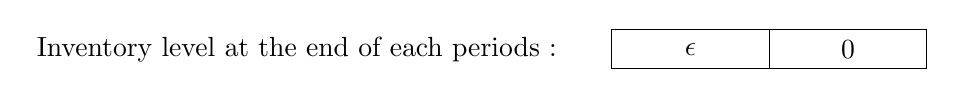
\begin{tikzpicture}
        \draw (-4, .25) node {Inventory level at the end of each periods : };
        \draw (0, 0) rectangle (2, .5) ++(-1, -.25) node {$\epsilon$};
        \draw (2, 0) rectangle (4, .5) ++(-1, -.25) node {$0$};
    \end{tikzpicture}
\end{center}

This allows to compute the total cost like so :
\[
    J = K + h\epsilon +
    \begin{cases}
        K &\textrm{if }\epsilon = 0\\
        0 &\textrm{if }\epsilon = d_2\\
        K &\textrm{if }\epsilon < d_2
    \end{cases}
    = \begin{cases}
        2K+h\epsilon&\textrm{if }\epsilon<d_2\\
        K+hd_2&\textrm{if }\epsilon = d_2
    \end{cases}
\]
Indeed, we always pay at least one order (which corresponds to the first order in period one) and the inventory cost for the remaining items after the first periods (which is $\epsilon$). In the case where $\epsilon = d_2$, we already have ordered enought products to fulfill both the demand of the first period and the demand of the second period, so we don't have to make another order and we don't pay for ordering nothing. Otherwise, we have to order again, so a new $K$ cost has to be paid. We then have two cases :
\begin{itemize}
    \item if $\epsilon < d_2$, then clearly, the minimum is reached by choosing $\epsilon = 0$
    \item if $\epsilon = d_2$, then minimum is $K+hd_2$
\end{itemize}

What this discussion means, is that, in order to choose a value for $\epsilon$ in order to minimize our cost, the only "good" decisions we can make are those of buying once for two periods or buying once at each period but in no case should we buy more in period one and buy again a smaller amount of goods in period two. That's the meaning of the Wagner-Within theorem.

\section{The Silver \& Mill Heuristic}

The Silver-Meal heuristic is a very simple algorithm which relies on the Wagner-Within theorem. It often drives the solution near the real solution which in most cases is acceptable. In fact, the algorithm finds a local minimum of the cost function (instead of a global minimum). Simply sumed up, this heuristic considers incrementing periods of time and looks at whether or not it would be a good idea to buy more than what is needed for that specific period of time. We know from the Wagner-Within theorem that if we buy more than needed, then whe should buy exactely the amount of good sufficient to satisfy the demand of the next period (otherwise it's not worth it). The algorithm computes a series of costs making this kind of assumptions until a local minimum is reached. Here is how it works : let $c(i)$ be the cost we would pay if, starting from the first period, we were to buy as many products as needed to statisfy up to the $i$-th period's demand. Clearly, the cost $c(1)$ is simply $K$ since we only make one order and don't pay for inventory since all our order is consumed by the demand in the first period ($a_1=d_1$). For the second period, the cost $c(2)$ is now the fixed price $K$, since we order once for two periods, to which we have to add the inventory cost we pay for the remaining inventory level after period one which corresponds exactely to $hd_2$. In order to compare $c(1)$ and $c(2)$, we'll focus on the \emph{average} cost that we pay per period of time instead of the absolute value. It holds then that $c(2) = \frac{K+hd_2}{2}$. Similarly, we can compute $c(3)$ as $c(3) = \frac{K + h(d_2+d_3) + hd_3}{3}=\frac{K+hd_2+2hd_3}{3}$ since we order once for the three subsequent periods of time and that we have to pay for inventory in period one (whose inventory level is then $d_2+d_3$) and in period two (whose inventory level is then $d_3$). Continuing like so, and searching for a local minimum, we get the Silver-Mill heuristic for choosing our actions. 

The general formula (which can be recursively demonstrated) for computing the coefficients $c(i)$s is given by 
\[ c(i) = \frac{K+hd_2+2hd_3+\hdots+(i-1)d_i}{i} \] Indeed, we assume paying once in period one, so we pay the order price $K$ just once, then we have to deal with inventory costs. The quantity $d_k$ will remain in the inventory untill period $k$ is reached. So the associated inventory cost is given by $(k-1)hd_k$ since we pay for having it in store in every preceding periods of time. 

The figure (\ref{periodic:local_minimum}) shows how the heuristic works. The algorithm continues to compute total costs (incrementing the number of periods considered) until a local minimum is found. In this example, our action will be to order in the first period for three periods of time since $c(3)$ is a local minimum of our function $J$. Note that, if we had continued to search for lower values we may have eventually found that (in this case), $c(5)$ was more advantageous from an economical point of view and we would have better done to buy all the products for 5 periods instead of four. But in general, this approach gives a really good approximation of the optimal value for the problem and, with respect to the simplicity of the algorithm, it often doesn't worth it to use more advanced and complex models. 

\begin{figure}
    \centering
    \begin{tikzpicture}[scale=1.4]
        \draw[<->] (0, 5.3) node [above] {$c(i)$} |- (7.3, 0) node [right] {$i$};

        \foreach \y in {1,...,5} { \draw[dotted] (0,\y) -- (7,\y); }
        \foreach \x in {1,...,7} { \draw[dotted] (\x,0) -- (\x,5); }

        \draw (1, 4.5) node [draw, cross out] (1) {} ++(0,.5) node {$c(1)$};
        \draw (2, 3) node [draw, cross out] (2) {} ++(0,.5) node {$c(2)$};
        \draw (3, 2) node [draw, cross out] (3) {} ++(0,.5) node {$c(3)$};
        \draw (4, 3.4) node [draw, cross out] (4) {} ++(0,.5) node {$c(4)$};
        \draw (5, 1.5) node [draw, cross out] (5) {} ++(0,.5) node {$c(5)$};
        \draw[dotted, thick] (1) -- (2) -- (3) -- (4) -- (5);

        \draw[red, ->, thick] (3,0) -- (3);
    \end{tikzpicture}
    \caption{\label{periodic:local_minimum}Silver-Mill heuristic example}
\end{figure}

\section{Analysis of the method}

In this last section of this chapter, we would like to discuss on the accuracy, or rather plausibility, of this method. In particular, we will have a look at what happens the demand for each period of time is homogeneous. Let $d$ be that demand. Using the previously established formula, it holds that :
\[
    \begin{split}
        c(n) &= \frac{K+hd+2hd+\hdots+(n-1)hd}{n}\\
            &= \frac{K+\sum_{i=1}^{n-1}ihd}{n}\\
            &= \frac{K+\frac{n(n-1)}{2}}{n}\\
            &= \frac{K}{n} + \frac{nhd}{2} - \frac{hd}{2}
    \end{split}
\]
and let us relax our problem considering the function $c(x)$ where $x$ is no longer discrete but continuous. Derivating this function, we get 
\[
    \begin{cases}
        \frac{dc}{dx} &= -\frac{K}{n^2} + \frac{hd}{2}\\
        \frac{d^2c}{dx^2} &= \frac{K}{n^3} > 0, \forall x\in\mathbb R
    \end{cases}
\]
The second derivative being greater than zero for any $x$ means that the function $c$ is convex. Knowing that, it is legit to compute the minimum of this function by truncating the solution of $\nabla c = 0$ to find the actual minimum of the non-relaxed problem (where $x\in\mathbb N$). Solving this equation we get : \[ \frac{dc}{dx} = 0 \Leftrightarrow x^* = \sqrt\frac{2K}{hd} \]
And since $Q = dn^*$, it holds that \[ Q = dx^* = \sqrt\frac{2kd}h  \] which is the exact same formula which we found in the first part of this course in the deterministic model. 